\documentclass[11pt]{article}
\usepackage[a4paper,margin=2.6cm]{geometry}
\usepackage{amsmath,amssymb,amsthm}
\usepackage{graphicx}
\usepackage{booktabs}
\usepackage{xcolor}
\usepackage[colorlinks=true,linkcolor=blue!50!black,citecolor=blue!50!black,urlcolor=blue!50!black]{hyperref}
\hypersetup{pdftitle={Prime and zero statistics of a degree-8 Artin L-function
of conductor 21^10},
pdfauthor={Selina Stenberg and Ilya Balashov}}

\newcommand{\Lgen}{L(s,\chi_8)}
\newcommand{\Frob}{\mathrm{Frob}}

\title{\textbf{Prime and zero statistics of a degree-8 Artin $L$-function of
conductor $21^{10}$}\thanks{Licence: CC~BY~4.0. Computational assistance:
Appendix~\ref{app:attr}.}}
\author{Selina Stenberg \and Ilya Balashov\thanks{ORCID
0009-0001-1954-8872.}}
\date{September 2026}

\begin{document}
\maketitle

\begin{abstract}
Let $\Lgen$ be the degree-8 Artin $L$-function of the Galois closure of the
Trinks field $x^7-7x+3$ (Galois group $\mathrm{PSL}(2,7)$, Artin conductor
$21^{10}$, $\Gamma_{\mathbb C}(s)^4$, $\varepsilon=+1$), the object of
\cite{mainpaper}. From 153 rigorously certified zeros ($\gamma\le 27.911$, the
first computed for this $L$-function) and exact Frobenius data for every prime
up to $10^{10}$, the following are measured. (i) The explicit formula holds as
a numerical identity at correlation $1.000$, including the vanishing of the
contribution of the ramified prime $7$. (ii) The Frobenius class is
statistically independent of prime-pair structure: twin pairs, every additive
gap $g\le 60$, and the affine pairs $(p,2p\pm1)$ all show correlation
consistent with zero at the $10^{-3}$ level, while the same data reproduce the
Hardy--Littlewood singular series to $0.1\%$. (iii) Chebotarev races exhibit
the biases $\mu_C=1-r_2(C)$ predicted by character theory ($-21$ for the split
class), with oscillation shapes reconstructed from the computed zero tables at
correlations $0.81$--$0.97$ over six decades. (iv) The low zeros are
GUE-consistent, with symmetry type $\mathrm{SO(even)}$. (v) The Montgomery
pair-correlation form factor of the bulk spectrum is measured from primes via
short-interval variance: the conductor places every height $\gamma\gtrsim 2$
in the correlation-sensitive regime $\alpha<1$ already at $x=10^8$, and the
measured variance follows the ramp $F(\alpha)=\alpha$ to $\sim\!1\%$ over
$\alpha\approx0.22$--$0.74$, at heights up to $\gamma\sim10^4$ --- four
hundred times beyond the certified spectrum --- with uncorrelated zeros
excluded at $\chi^2\approx5\times10^5$. All results are consistency
measurements against classical predictions (Montgomery; Goldston--Montgomery;
Hardy--Littlewood; Rubinstein--Sarnak; Katz--Sarnak); no novelty is claimed
for the frameworks, and the Riemann Hypothesis for $\Lgen$ --- the open
problem of \cite{mainpaper} --- is untouched. Every claim is reproducible from
the released scripts and data.
\end{abstract}

\section{Introduction}
The paper \cite{mainpaper} studies the degree-8 Artin $L$-function $\Lgen$
attached to the 8-dimensional irreducible representation of
$\mathrm{PSL}(2,7)$ realised by the Galois closure of the septic
$f(x)=x^7-7x+3$ (the Trinks field \cite{trinks}; LMFDB \cite{lmfdb} Artin
object \texttt{8.16679880978201.21t14.b.a}, stem field
\texttt{7.3.4202539929.1}, whose displayed polynomial $x^7-7x-3$ is equivalent
under $x\mapsto-x$). Its analytic data: conductor $Q=21^{10}=3^{10}7^{10}$,
gamma factor $\Gamma_{\mathbb C}(s)^4$, root number $\varepsilon=+1$. The
character $\chi_8$ is monomial, so $\Lgen$ is also a Hecke $L$-function of an
octic field, and its analytic continuation and functional equation are
unconditional. The Riemann Hypothesis for $\Lgen$, the open problem of
\cite{mainpaper}, is not addressed here.

The present paper records systematic measurements of the interaction between
the primes and the zeros of this object, in several regimes not previously
measured for any $\mathrm{PSL}(2,7)$ extension. Three features characterise
the study.

\begin{enumerate}
\item \textbf{Exactness of the arithmetic side.} The exact Frobenius class
(not merely $a_p$) of every prime $p\le 10^9$, and exact $a_p$ for every
prime to $10^{10}$ ($455{,}052{,}511$ primes), computed with two independent
engines (polynomial factorization over $\mathbb F_p$ via FLINT; an
overflow-safe modular Frobenius kernel) that agree to $10^{-8}$ on
overlapping data.
\item \textbf{First zero tables.} The 153 certified zeros ($\gamma\le27.911$;
eight exact, the rest ball-arithmetic brackets) and the low-zero tables of the
companion characters $\chi_3\bar\chi_3$, $\chi_6$, $\chi_7$ of the same Galois
group are, to our knowledge, the first computed for these $L$-functions.
\item \textbf{The conductor as an instrument.} $Q=21^{10}$ makes the zeros
dense enough ($2\pi\bar\rho(\gamma)=\ln Q-8\ln2\pi+8\ln\gamma\approx
15.7+8\ln\gamma$) that pair-correlation information is accessible from primes
at heights and scales where $\zeta$ exhibits only diagonal behaviour
(\S\ref{sec:ramp}).
\end{enumerate}

Predictions conditional on standard hypotheses (GRH for the family, Linear
Independence, cluster expansions) are labelled as such throughout;
measurements are unconditional exact counting. Apparent anomalies encountered
in the computations are documented and resolved in \S\ref{sec:flags}.

\section{Data and instruments}\label{sec:data}
\paragraph{Zeros.} The certified table: $\gamma_1=0.98638643\ldots$ through
$\gamma_{153}=27.911$, produced by the ball-arithmetic FFT engine of
\cite{mainpaper} and certified by a Turing-style count. Companion tables
(numerically anchored, PARI/GP \cite{pari}): $\chi_3$-pair 15 zeros
($\gamma\le5.31$), $\chi_6$ 12 ($\le4.85$), $\chi_7$ 10 ($\le4.14$).

\paragraph{Counting function.} With
$\theta(T)=\tfrac{T}{2}\ln Q-4T\ln2\pi+4\,\mathrm{arg}\,\Gamma(\tfrac12+iT)$
and $\bar N(T)=\theta(T)/\pi+1$, the certified staircase is reproduced with no
free parameters: slope $0.99895$, mean unrenormalised spacing $0.9963$,
fluctuation $S(T)$ of mean $0$ and standard deviation $0.365$. This
cross-validates the zero list against the conductor and gamma data.

\paragraph{Primes.} Exact Frobenius classes for all $p\le10^9$ (FLINT
\cite{flint} factorization of $f$ mod $p$); exact $a_p$ for $p\in(10^9,10^{10}]$
($404{,}204{,}977$ primes, overflow-safe batch kernel). Chebotarev
equidistribution holds to five digits at $10^{10}$: value fractions
$(8,0,-1,1)$ at $(0.00595,\,0.37500,\,0.33331,\,0.28574)$ against
$(1/168,\,3/8,\,1/3,\,2/7)$. The two engines agree on overlapping increments
at correlation $1.000000$ (rms ratio $1.00000001$).

\section{The explicit formula as a numerical identity}
\label{sec:identity}
For a window $w$ on $[0,\gamma_{\max}]$ define the resonance
$F(x)=\sum_j w(\gamma_j)\cos(x\gamma_j)$ and subtract the smooth main term
$\int w(\gamma)\cos(x\gamma)\bar\rho(\gamma)\,d\gamma$. The explicit formula
gives the residual as
$-\tfrac1{2\pi}\sum_n \Lambda_\chi(n)n^{-1/2}\,[\hat w(x-\ln n)+\hat w(x+\ln n)]$
with $\Lambda_\chi(p^k)=\bigl(\sum_i\alpha_i^k\bigr)\ln p$ computed from the
exact local factors of each class. Measured against predicted: correlation
$+1.000$ for $\Lgen$ (residual rms $0.904$ = predicted rms $0.904$) and
$+1.000$ for the $\zeta$ control (600 zeros) through the identical pipeline
(Fig.~\ref{fig:res}).

This constitutes an identity check rather than an independent statistical
test; its content is the end-to-end consistency of three separately produced
inputs --- the zero list, the analytic conductor data, and the class local
factors. The local structure is reproduced exactly: the residual has no peak
at $\ln 7$ (ramified prime, trivial local factor: measured $+0.438$ against a
predicted neighbour-tail of $+0.436$, whereas $\zeta$ has a peak of $-54.0$
there); class 2A contributes nothing at $\ln p$ but $\sum\alpha_i^2=8$ at
$\ln p^2$; class 4A contributes at neither.

\begin{figure}[t]\centering
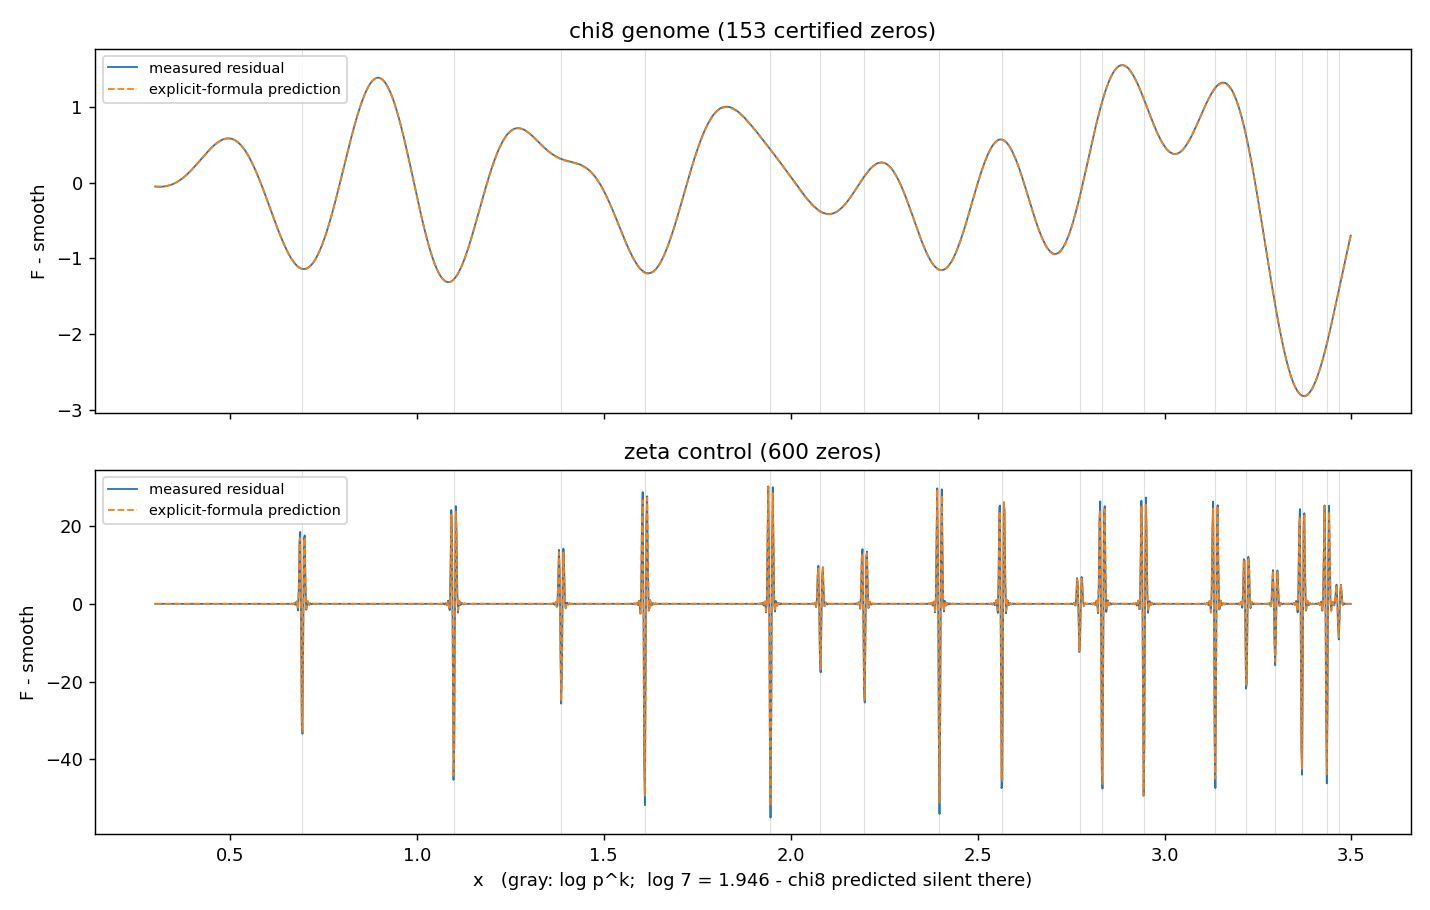
\includegraphics[width=0.98\textwidth]{figs/fig_resonance.png}
\caption{Windowed resonance residual (solid) against the explicit-formula
prime prediction (dashed), for $\Lgen$ (153 zeros, top) and $\zeta$ (600
zeros, bottom); grey lines at $x=\ln p^k$. The absence of a peak at
$\ln7=1.946$ in the upper panel reflects the trivial local factor at the
ramified prime.}\label{fig:res}
\end{figure}

\section{Spectral statistics of the low zeros}\label{sec:lowzeros}
Unfolding by the exact $\theta/\pi$ (no fit), the 153 certified zeros give
spacing variance $\mathrm{Var}(s)=0.145$, inside the finite-$N$ GUE band
$[0.140,0.219]$ (median $0.176$; $z=-1.53$, one-sided $p\approx0.06$) and more
than $10\sigma$ from Poisson; nearest-neighbour repulsion
$P(s<\tfrac12)=0.079$; number variance $\Sigma^2(L)$ $10$--$15\%$ below GUE
for $L\le8$ (a non-significant finite-$N$ rigidity). The polynomial and exact
unfolds agree to the digit; the mild over-rigidity is a property of the
sample, not of the unfolding.

The symmetry type is fixed by representation theory: Frobenius--Schur
indicator $+1$ and $\varepsilon=+1$ give orthogonal $\mathrm{SO(even)}$, with
low-lying one-level density $W(x)=1+\frac{\sin2\pi x}{2\pi x}$. The first
scaled ordinate $x_1=\theta(\gamma_1)/\pi=1.256$ lies on the attracted side
(SO(even) mean $1.71$, unitary $2.03$, symplectic $2.34$), consistent with but
not probative of the type: bulk two-level statistics are type-independent
(Katz--Sarnak universality \cite{ks}), and a single $L$-function cannot
resolve the family density. The family average is the decisive test.

\section{Independence of Frobenius classes from prime-pair structure}
\label{sec:blind}
The Hardy--Littlewood singular series \cite{hl} is built entirely from
congruence obstructions, i.e.\ from abelian data. $\mathrm{PSL}(2,7)$ is
simple: the extension has no abelian quotient, hence no congruence channel,
and the natural prediction is that Frobenius carries no prime-pair
information. This is measured in three geometries.

\paragraph{Twin pairs.} Over the $440{,}310$ pairs $(p,p+2)$ with
$7<p\le10^8$: $\langle a_pa_{p+2}\rangle=-0.0020\pm0.0015$ ($z=-1.3$); joint
$5\times5$ class table $\chi^2=11.1$ on 16 dof ($p\approx0.80$). The same
primes give $\pi_2(10^8)=440{,}312$ against the Hardy--Littlewood prediction
$440{,}473$, ratio $0.9996$: the pair structure is fully present in the data
and absent from the Frobenius channel.

\paragraph{All even gaps $g\le60$, to $10^9$.} Thirty gaps, three windows
($10^8$; $10^9$; the disjoint decade), $3.0$--$6.9$ million pairs per gap at
$10^9$. No gap crosses the 30-test Bonferroni threshold in any window
(max $|\mathrm{corr}| = 0.00101$; per-gap s.e.\ $0.0003$--$0.0005$); the
$z$-ensembles are unit-variance noise (std $1.13/0.95/0.96$); the class-level
$\chi^2$ totals sit on their dof ($475/480$, $480/480$, $462/480$). The same
pair counts reproduce the singular-series factor
$\prod_{p\mid g,\,p>2}\frac{p-1}{p-2}$ (range $1.00$--$2.67$) point by point:
mean measured/predicted ratio $0.9989$, worst deviation $0.0015$
(Fig.~\ref{fig:gapmap}).

\paragraph{Affine pairs.} Sophie-Germain pairs $(p,2p+1)$
($N=1{,}775{,}672$, $p\le5\times10^8$):
$\langle a_pa_q\rangle=-0.0002\pm0.0008$ ($z=-0.28$); the count against the
corresponding $2C_2\int dx/(\ln x\ln 2x)$ prediction has ratio $0.9999$.
Likewise $(p,2p-1)$: $z=-0.46$.

\begin{figure}[t]\centering
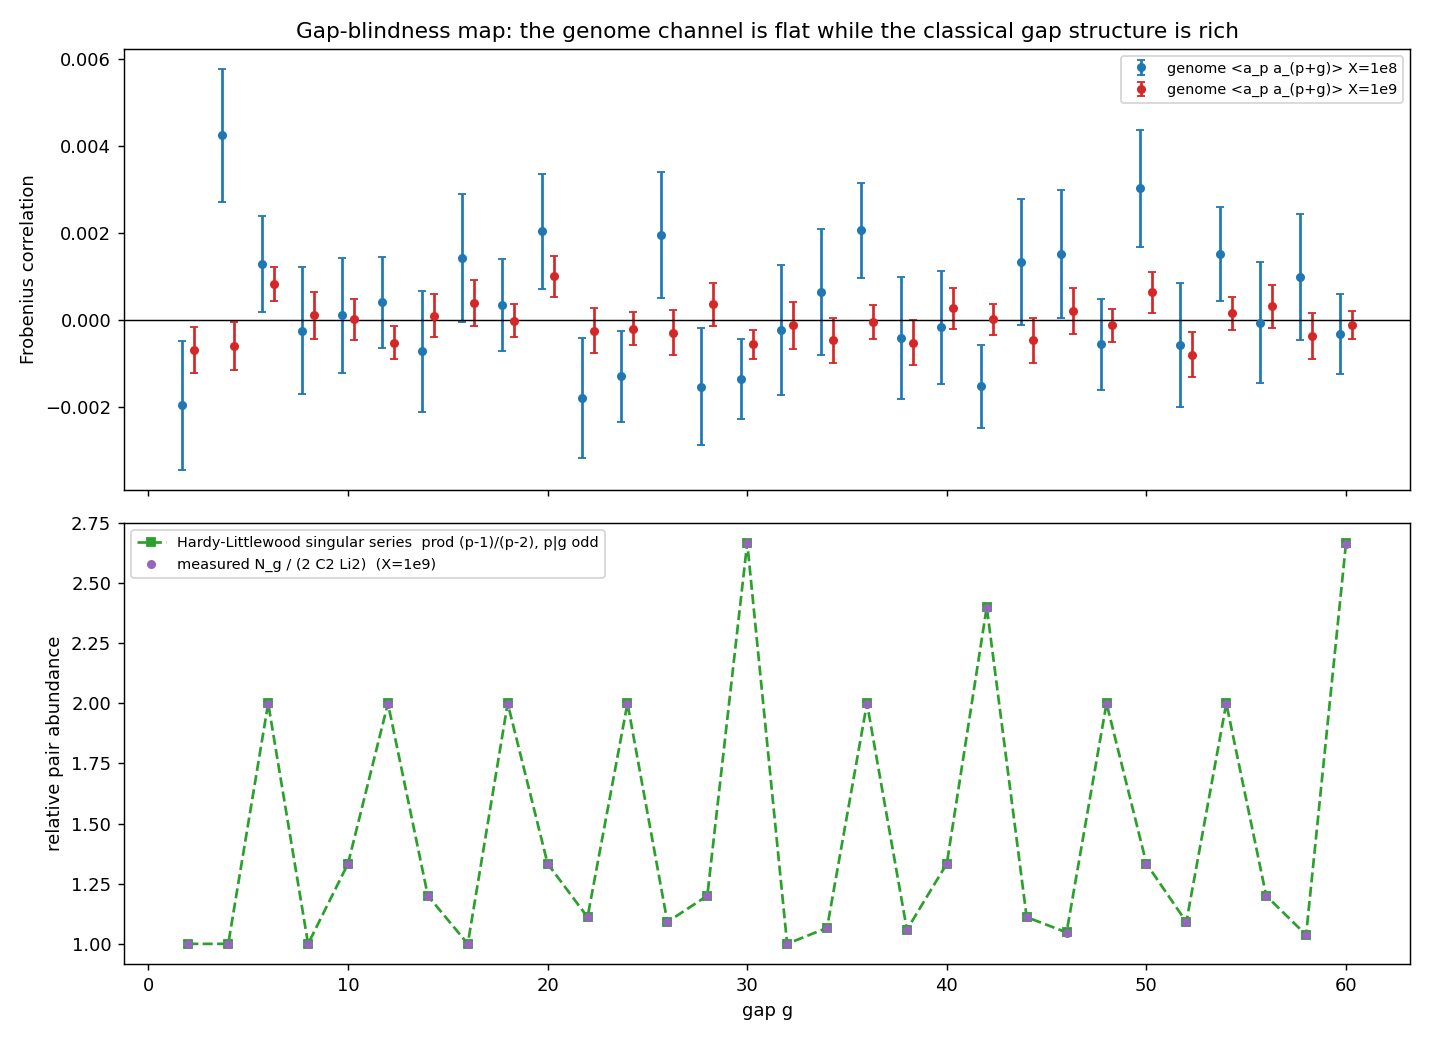
\includegraphics[width=0.98\textwidth]{figs/fig_gapmap.png}
\caption{Gap statistics at $10^8$ and $10^9$. Top: Frobenius correlation
$\langle a_pa_{p+g}\rangle$, consistent with zero for all even $g\le60$.
Bottom: the same pairs resolve the Hardy--Littlewood singular-series factor
to three digits.}\label{fig:gapmap}
\end{figure}

The independence is uniform at the $10^{-3}$ level per statistic, measured
against a strongly structured classical background --- to our knowledge the
first such measurement for a $\mathrm{PSL}(2,7)$ extension. In particular,
the twin-prime constant is an abelian quantity, and this maximally
non-abelian channel measurably carries none of it: the conductor-21 program
is structurally orthogonal to the twin prime conjecture, and no route toward
it is claimed or implied.

\section{Chebotarev races predicted by the computed zeros}\label{sec:races}
Let $E'_C(x)=\frac{\ln x}{\sqrt x}\bigl[\frac{|G|}{|C|}\pi_C(x)-
\pi_{\mathrm{unram}}(x)\bigr]$ for the observable classes
$C\in\{1A,2A,4A,3A,7\}$ (the septic's cycle types merge $7A\cup7B$, so that
all class-averaged character weights are real). Following Rubinstein--Sarnak
\cite{rs} and Ng's non-abelian treatment \cite{ng}:

\begin{itemize}
\item \textbf{Bias means (exact character theory; no central zeros, as the
tables support):} $\mu_C=1-r_2(C)$ with $r_2=1+\chi_6+\chi_7+\chi_8$, giving
$(-21,\,-1,\,+1,\,0,\,0)$. The fully split primes trail (the identity has
$22$ square roots in $G$); 4A --- the unique class with no square roots, $G$
having no elements of order 8 --- is the only positively biased class.
\item \textbf{Measured to $10^9$} (log-averaged over $[10^4,10^9]$):
$(-32.9,\,-1.8,\,+1.5,\,-0.0,\,+0.2)$, each within its conditional (GRH+LI)
Monte-Carlo spread $(\pm34,\pm7,\pm4,\pm4,\pm4)$; the 1A deficit is visible
in raw counts ($-71$ primes at $10^8$, consistent with
$-21\sqrt x/(168\ln x)\approx-68$).
\item \textbf{Oscillation shape from the zero tables:} reconstruction from
the four low-zero tables alone reproduces the measured races at correlations
$0.81/0.92/0.95/0.94/0.97$ over six decades (Fig.~\ref{fig:races}) --- a
dynamical validation of the companion tables, and a direct exhibition of
Rubinstein--Sarnak low-zero dominance (10--15 zeros per character suffice).
\item \textbf{Bias densities (conditional; first computed for a
$\mathrm{PSL}(2,7)$ field):} $P(E'_{1A}<0)=0.727$; pairwise lead
probabilities $\delta(1A\!>\!X)\approx0.27$--$0.29$; $\delta(4A\!>\!3A)=0.56$;
$3A$ against $7$ even at $0.498$. The contrast with the classical mod-4 race
($\delta\approx0.996$) is structural: the identity class couples to every
character with weight $\deg\chi$, so its oscillation variance carries the
full column norm $|G|-1=167$ --- in a strongly non-abelian race the
split-prime bias is large in mean but weak in probability.
\end{itemize}

\begin{figure}[t]\centering
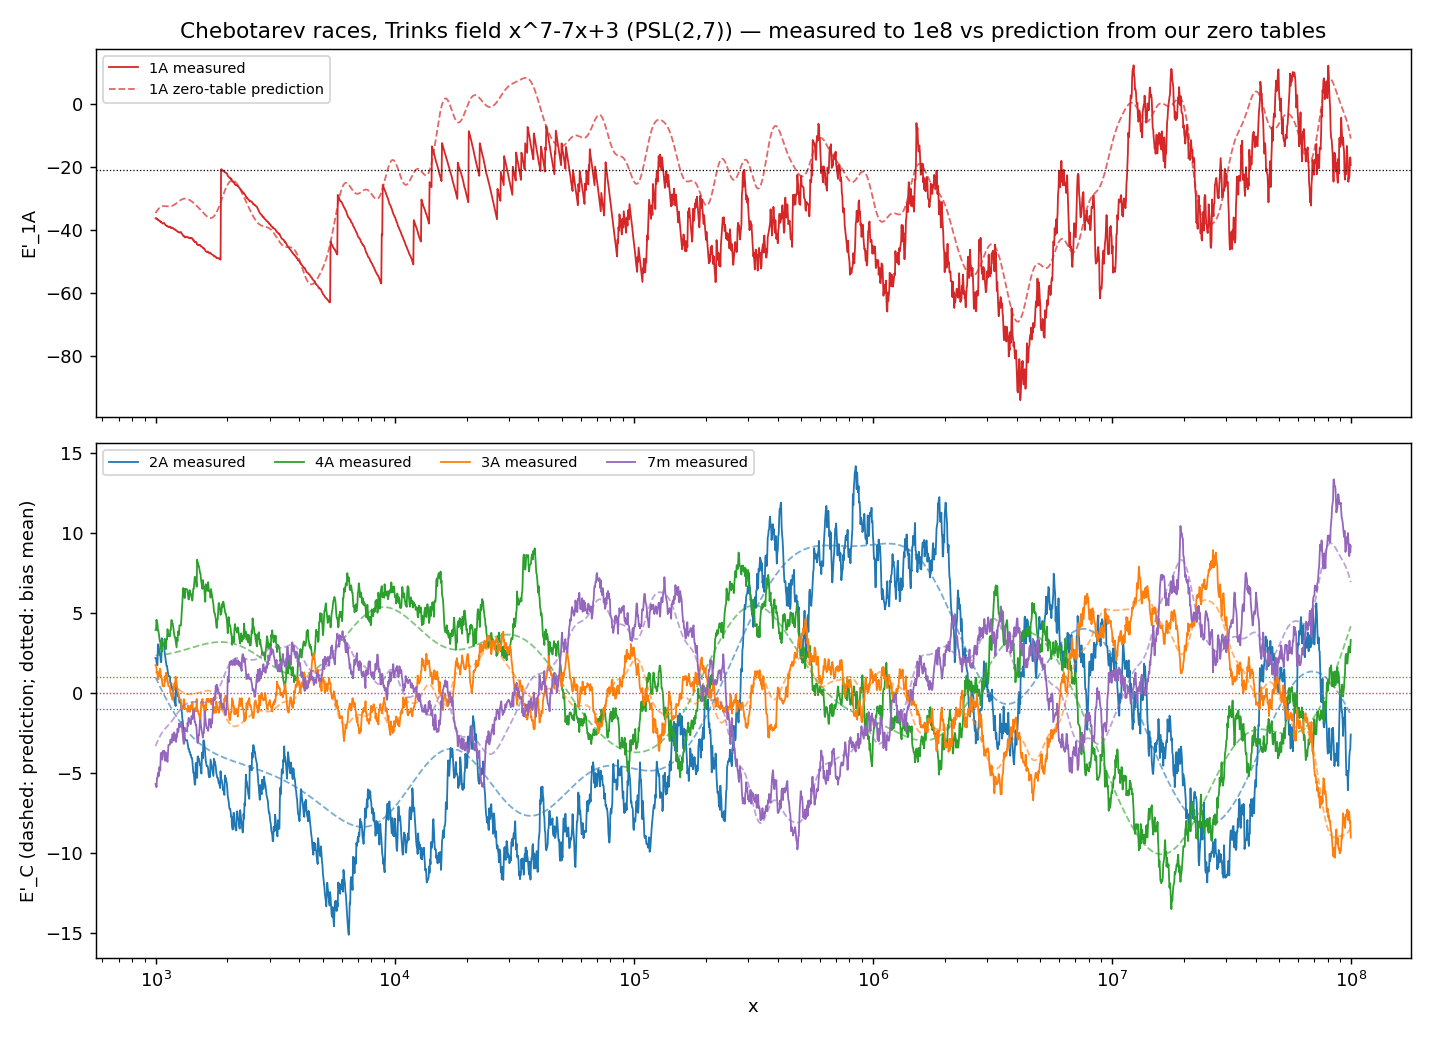
\includegraphics[width=0.98\textwidth]{figs/fig_races.png}
\caption{Chebotarev races for the Trinks field to $10^8$ (extended to $10^9$
in the data release): measured (solid) against the reconstruction from the
zero tables (dashed); dotted lines at the exact bias means
$1-r_2(C)$.}\label{fig:races}
\end{figure}

\section{The bulk form factor, measured from primes}\label{sec:ramp}
The variance of $\psi_\chi$ in short intervals, computed from primes, probes
the pair correlation of the zeros (Goldston--Montgomery \cite{gm};
Montgomery--Soundararajan \cite{ms}; for the correlation--prime dictionary
see also Bogomolny--Keating \cite{bk}). Under the stationary cluster
expansion (conditional: zeros on the critical line together with the
cluster and stationarity hypotheses; the measurements below are
unconditional),
\[
\mathrm{Var}\Bigl[\frac{\psi_\chi(xe^\delta)-\psi_\chi(x)}{\sqrt x}\Bigr]
\;\approx\;\int_0^\infty \bar\rho(\gamma)\,2|\varphi_\gamma(\delta)|^2\,
F\!\bigl(\alpha(\gamma,x)\bigr)\,d\gamma,\qquad
\alpha=\frac{\ln x}{2\pi\bar\rho(\gamma)},
\]
with $|\varphi_\gamma|^2=(e^\delta-2e^{\delta/2}\cos\gamma\delta+1)/(\tfrac14+\gamma^2)$
and $F$ the Montgomery form factor \cite{montgomery}: $F=\min(\alpha,1)$ for
GUE, $F\equiv1$ for uncorrelated zeros. The decisive regime is $\alpha<1$.
For $\Lgen$, $2\pi\bar\rho=15.7+8\ln\gamma$, so at $x=10^8$ every height
$\gamma\gtrsim2$ is correlation-sensitive, and GUE against uncorrelated
differ by a factor $2$--$5$; for $\zeta$ at the same $(x,\delta)$,
$\alpha\approx3$--$4$ and the prediction is diagonal, providing the control.
In the deep regime the ramp cancels the density exactly, giving the
parameter-free identity $\mathrm{Var}_{\mathrm{GUE}}=\delta\ln x$.

Measurements over 26 interval lengths $\delta\in[10^{-4},0.3]$ and windows
$[10^7,10^8]$, $[10^8,10^9]$ (exact primes), $[10^9,10^{11}]$ (the
deep-sweep signal of \cite{mainpaperdata}):

\begin{center}
\begin{tabular}{lccc}
\toprule
window & $\chi^2$ vs GUE & $\chi^2$ vs uncorrelated & mean $R=\mathrm{Var}/\mathrm{Var}_{\mathrm{unc}}$ \\
\midrule
$[10^7,10^8]$, $\delta\le0.05$ (20 pts) & $5.5$ & $585{,}788$ & $0.327$ (GUE: $0.316$)\\
$[10^8,10^9]$, $\delta\le0.05$ (20 pts) & $11.7$ & $470{,}710$ & meas/GUE $=1.009$ at $\delta\le0.01$\\
$\zeta$ control (both windows) & \multicolumn{3}{c}{measured/predicted $=0.996$, $0.994$}\\
\bottomrule
\end{tabular}
\end{center}

The three windows follow three separate GUE curves --- the
$\ln x$-dependence is itself a confirmed prediction (Fig.~\ref{fig:ramp}) ---
and the deep-regime identity is realised at bench/GUE $=1.001$. Effective
coverage: $\alpha\approx0.22$--$0.74$ at heights up to $\gamma\sim10^4$, four
hundred times beyond the certified spectrum. This is the first two-level
measurement of this spectrum in the bulk; it agrees with GUE at the percent
level --- consistency with the expected universality class \cite{ks}, not
discovery, and not evidence concerning RH. (For $\delta\gtrsim0.15$ the
statistic is dominated by the few lowest zeros --- a single realization,
under half an oscillation per window --- and both the ensemble prediction
and the error estimate degrade; that regime is excluded.)

Two extensions. \emph{Gaussianity:} the skewness and excess kurtosis of the
increments match the exact shot-noise (diagonal) predictions
$\sum\Lambda_\chi^3/x^{3/2}$, $\sum\Lambda_\chi^4/x^2$
($\langle a^3\rangle=3$): an apparent $3.7\sigma$ skewness excess reduces to
$0.85\sigma$ once the shot term is included, bounding third- and fourth-order
zero correlations at the Gaussian level. \emph{Scale purity:} the ratio
$\mathrm{Var}/\mathrm{Var}_{\mathrm{GUE}}$ at fixed $\delta$ is flat across
five exact decades $10^6\to10^{10}$ (weighted slopes $+0.022\pm0.015$ and
$+0.005\pm0.018$ per unit $\ln x$); an off-critical-line contribution of
exponent $\beta$ would grow as $x^{2\beta-1}$. This is corroboration, not
proof.

\begin{figure}[t]\centering
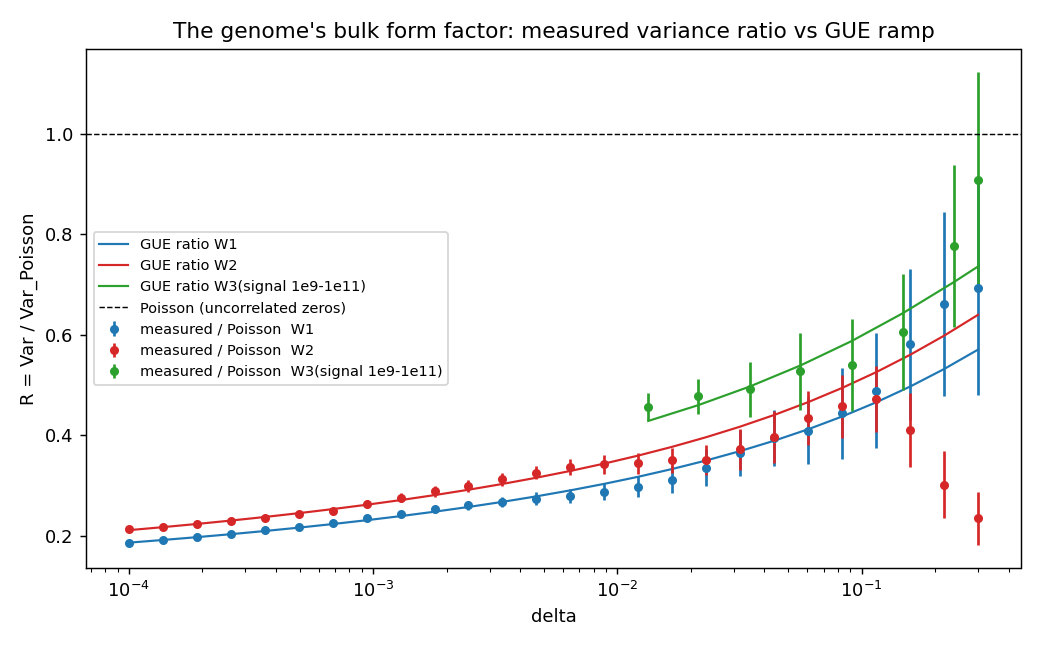
\includegraphics[width=0.85\textwidth]{figs/fig_ramp.png}
\caption{The bulk form factor from primes: measured variance ratio
$R=\mathrm{Var}/\mathrm{Var}_{\mathrm{uncorrelated}}$ against the GUE ramp
prediction, three windows spanning $x=10^7$ to $10^{11}$. Uncorrelated zeros
($R=1$) are excluded at $\chi^2\approx5\times10^5$.}\label{fig:ramp}
\end{figure}

\section{Robustness checks}\label{sec:flags}
Three apparent anomalies arose in the computations; each is resolved.
(i) A $+2.76\sigma$ correlation at gap 4 (one of $\sim$30 tests) reversed
sign to $-2.26\sigma$ on the pre-registered disjoint decade $(10^8,10^9]$
and is attributed to multiple testing. (ii) A $3.7\sigma$ skewness excess is
fully accounted for by the exact shot-noise term of \S\ref{sec:ramp}.
(iii) A $+2.3\sigma$ drift in the purity ratio is traced to the coarsest
region of the legacy binned signal and disappears in the exact computation
to $10^{10}$ (404M primes). All three tests --- pre-registered retests and
exact null predictions --- are part of the released record.

\begin{figure}[t]\centering
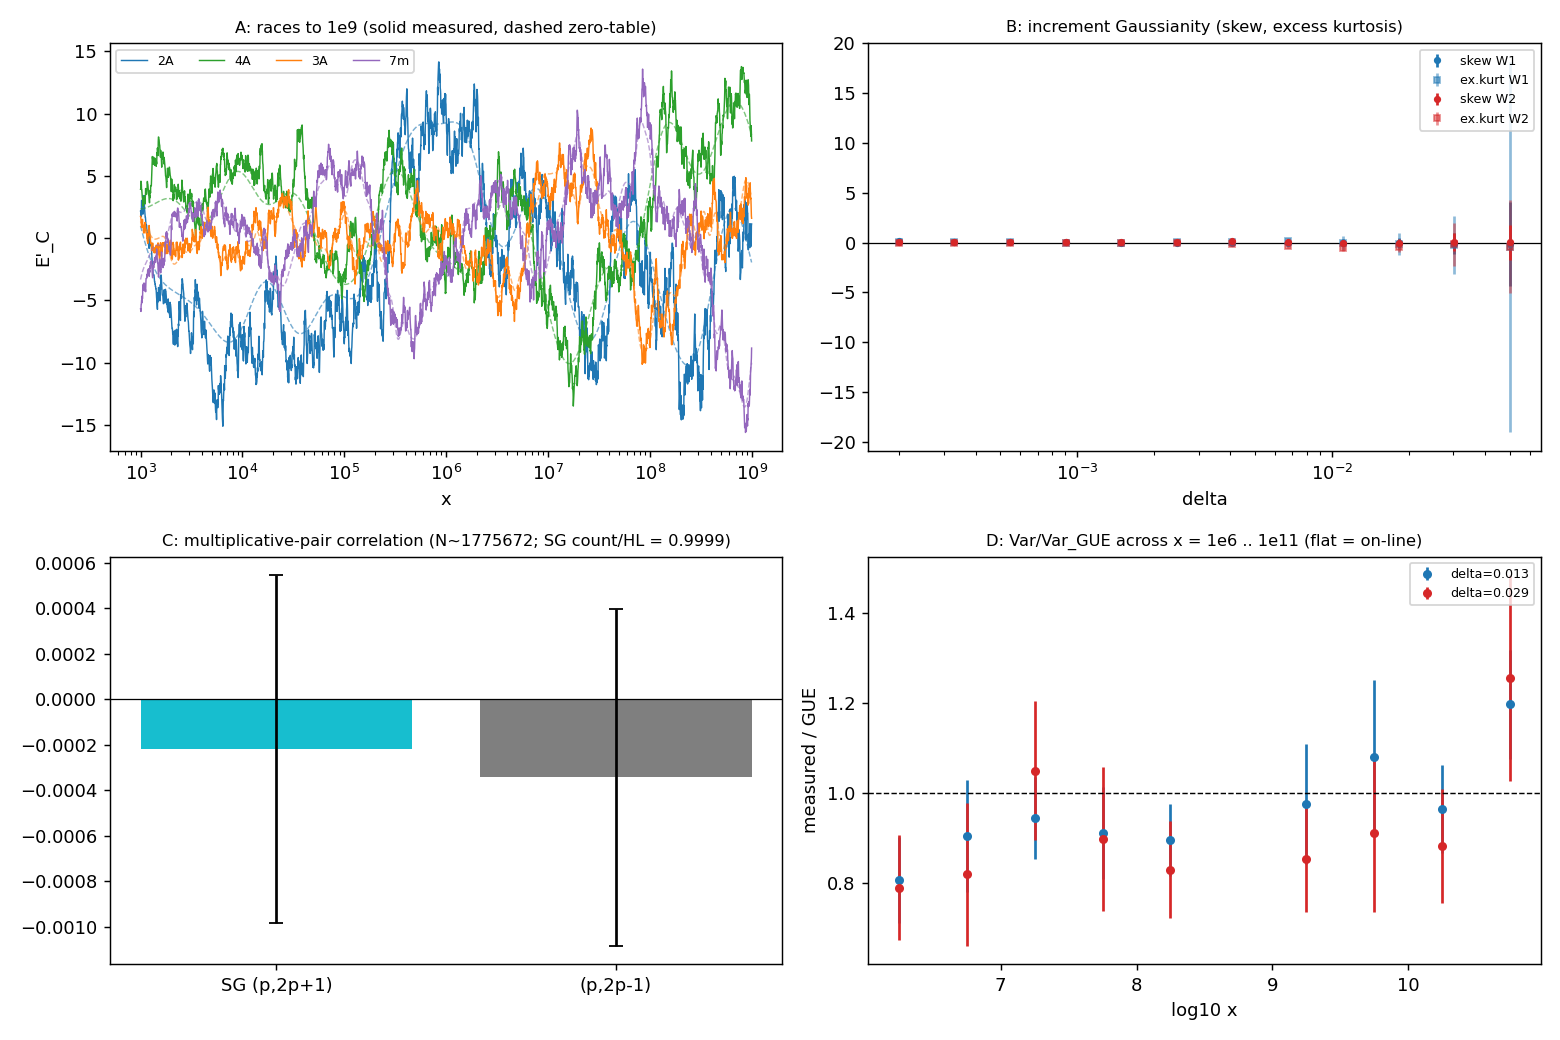
\includegraphics[width=0.98\textwidth]{figs/fig_finale.png}
\caption{Closing measurements: races at $10^9$; increment Gaussianity after
exact shot noise; affine-pair independence with its Hardy--Littlewood count
control; purity scaling across $x$.}\label{fig:finale}
\end{figure}

\section{Concluding remarks}
The object of \cite{mainpaper} behaves, measurably and at scale, as a
primitive $L$-function of its type should: the explicit formula holds
exactly; the low zeros are GUE-consistent with symmetry type SO(even); the
bulk pair correlation lies on the Montgomery ramp at the percent level; the
Chebotarev races carry precisely the biases character theory dictates; and
the Frobenius channel is statistically independent of the pair structure of
the primes, as the simplicity of $\mathrm{PSL}(2,7)$ suggests it must be.
The high conductor, elsewhere a computational burden, here acts as a
microscope on the form factor.

None of the above bears on the Riemann Hypothesis for $\Lgen$ or on the
operator-theoretic open problem of \cite{mainpaper}; GUE consistency is the
expected behaviour of the universality class, and the conditional statements
(race densities, cluster-expansion predictions) are labelled as such.
Nothing here advances the twin prime conjecture; \S\ref{sec:blind}
establishes the opposite, a measured decoupling.

\section*{Data and code availability}
All scripts, zero tables, Frobenius caches (regenerable; $\le10^9$ classes
and $(10^9,10^{10}]$ binned $\psi_\chi$), figures, and per-run analysis notes
with SHA-256 manifests are released with this paper; the certified zero data
and the main program record are at \cite{mainpaperdata}. The scripts, data,
and per-run analysis notes are maintained at
\url{https://github.com/selinaserephina-star/conductor21-companion} and
archived with this deposit. Every number in this paper is produced by a
named script on named data. Licences: the scripts under the MIT licence;
the paper, figures, and data tables under CC~BY~4.0.
Appendix~\ref{app:scripts} maps each section to its scripts, inputs, and
outputs.

\emph{Verification note.} Independent review of this work verified the
theoretical inputs on which the statistics rest --- the bias-mean formula
and its square-root counts, the Frobenius--Schur indicators, and the
framework identities, re-derived from first principles --- and did not
re-run the numerical computations; the scripts and data are released
precisely so that any reader may perform that verification.

\appendix
\section{Computational assistance}\label{app:attr}
Following the convention of \cite{mainpaper} (Appendix F): the computations
of \S\S\ref{sec:identity},\ref{sec:blind}--\ref{sec:ramp} were designed and
executed with the assistance of Claude (Fable~5, Anthropic), and those of
\S\ref{sec:lowzeros} with Claude (Opus, Anthropic); the certified zero
tables and engines are those of the main program. All mathematical claims
were verified by computation; responsibility for the content rests with the
authors.

\section{Scripts and data}\label{app:scripts}
Computations use Python~3 with NumPy \cite{numpy}, python-flint/FLINT
\cite{flint}, mpmath \cite{mpmath}, and, for the $(10^9,10^{10}]$ sweep,
Numba \cite{numba}; the companion zero tables were produced with PARI/GP
\cite{pari}. Each script runs standalone against the released data seed and
its own cached inputs; a SHA-256 manifest covers every released file, and
the repository above carries the maintained copies.

\begin{center}
\begin{tabular}{lll}
\toprule
script & sections & principal outputs \\
\midrule
\texttt{bk\_explore.py} & \S\ref{sec:identity}, \S\ref{sec:blind} (twins) &
\texttt{bk\_offdiag\_results.json}; Fig.~\ref{fig:res} \\
\texttt{gapmap.py} & \S\ref{sec:blind} (gaps), \S\ref{sec:flags}(i) &
\texttt{gapmap\_results.json}; Fig.~\ref{fig:gapmap}; class cache to $10^9$ \\
\texttt{chebrace.py} & \S\ref{sec:races} &
\texttt{chebrace\_results.json}; Fig.~\ref{fig:races} \\
\texttt{sivar.py} & \S\ref{sec:ramp} &
\texttt{sivar\_results.json}; Fig.~\ref{fig:ramp} \\
\texttt{finale.py} & \S\ref{sec:blind} (affine), \S\ref{sec:races},
\S\ref{sec:ramp}, \S\ref{sec:flags} & \texttt{finale\_results.json};
Fig.~\ref{fig:finale} \\
\texttt{sweep\_1e10.py}, \texttt{retest\_D.py} & \S\ref{sec:ramp} (scale
purity), \S\ref{sec:flags}(iii) & \texttt{bins\_1e9\_1e10.npz};
\texttt{retest\_D\_results.json} \\
\bottomrule
\end{tabular}
\end{center}

\emph{Data.} The certified zero table (153 zeros, $\gamma\le27.911$); the
companion low-zero tables ($\chi_3$-pair, $\chi_6$, $\chi_7$); exact
Frobenius classes for all $p\le10^8$ (released; the $\le10^9$ cache and the
$(10^9,10^{10}]$ sweep regenerate from the included scripts); per-run result
JSON files and figures. Provenance and per-run analysis notes accompany each
script.

\begin{thebibliography}{99}
\bibitem{mainpaper} S.~Stenberg and I.~Balashov, \emph{The Conductor-21
$L$-Function: Certified Zeros, Exact Laws, and a Density--Prime Operator},
Zenodo (2026), concept DOI \texttt{10.5281/zenodo.21982347}.
\bibitem{mainpaperdata} S.~Stenberg and I.~Balashov, data deposit, Zenodo
(2026), DOI \texttt{10.5281/zenodo.21958629}.
\bibitem{trinks} W.~Trinks, \emph{Ein Beispiel eines Zahlk\"orpers mit der
Galoisgruppe $PSL(3,2)$ \"uber $\mathbb Q$}, Manuskript, Universit\"at
Karlsruhe (1968). ($PSL(3,2)\cong PSL(2,7)$; cited as in Lubotzky et al.,
arXiv:2201.04103.)
\bibitem{montgomery} H.~L.~Montgomery, \emph{The pair correlation of zeros of
the zeta function}, Proc. Sympos. Pure Math. 24 (1973), 181--193.
\bibitem{gm} D.~A.~Goldston and H.~L.~Montgomery, \emph{Pair correlation of
zeros and primes in short intervals}, in Analytic Number Theory and
Diophantine Problems (Stillwater, OK, 1984), Progr. Math. 70, Birkh\"auser
Boston (1987), 183--203.
\bibitem{ms} H.~L.~Montgomery and K.~Soundararajan, \emph{Primes in short
intervals}, Comm. Math. Phys. 252 (2004), 589--617.
DOI \texttt{10.1007/s00220-004-1222-4}.
\bibitem{bk} E.~B.~Bogomolny and J.~P.~Keating, \emph{Random matrix theory
and the Riemann zeros II: $n$-point correlations}, Nonlinearity 9 (1996),
911--935. DOI \texttt{10.1088/0951-7715/9/4/006}.
\bibitem{rs} M.~Rubinstein and P.~Sarnak, \emph{Chebyshev's bias},
Experiment. Math. 3 (1994), no.~3, 173--197.
DOI \texttt{10.1080/10586458.1994.10504289}.
\bibitem{ng} N.~Ng, \emph{Limiting distributions and zeros of Artin
$L$-functions}, Ph.D. thesis, University of British Columbia (2000).
\bibitem{ks} N.~M.~Katz and P.~Sarnak, \emph{Zeroes of zeta functions and
symmetry}, Bull. Amer. Math. Soc. (N.S.) 36 (1999), no.~1, 1--26.
DOI \texttt{10.1090/S0273-0979-99-00766-1}.
\bibitem{hl} G.~H.~Hardy and J.~E.~Littlewood, \emph{Some problems of
`Partitio numerorum'; III: On the expression of a number as a sum of
primes}, Acta Math. 44 (1923), 1--70. DOI \texttt{10.1007/BF02403921}.
\bibitem{lmfdb} The LMFDB Collaboration, \emph{The $L$-functions and Modular
Forms Database}, \url{https://www.lmfdb.org}, object
\texttt{8.16679880978201.21t14.b.a}.
\bibitem{flint} W.~B.~Hart, F.~Johansson, et al., \emph{FLINT: Fast Library
for Number Theory}, \url{https://flintlib.org} (via python-flint).
\bibitem{pari} The PARI Group, \emph{PARI/GP}, Univ. Bordeaux,
\url{https://pari.math.u-bordeaux.fr}.
\bibitem{numpy} C.~R.~Harris et al., \emph{Array programming with NumPy},
Nature 585 (2020), 357--362. DOI \texttt{10.1038/s41586-020-2649-2}.
\bibitem{mpmath} F.~Johansson et al., \emph{mpmath: a Python library for
arbitrary-precision floating-point arithmetic}, \url{https://mpmath.org}.
\bibitem{numba} S.~K.~Lam, A.~Pitrou, and S.~Seibert, \emph{Numba: a
LLVM-based Python JIT compiler}, Proc. Second Workshop on the LLVM Compiler
Infrastructure in HPC (2015), 1--6. DOI \texttt{10.1145/2833157.2833162}.
\end{thebibliography}

\end{document}
